\section{Method selection and architecture}

\begin{frame}{Choosing an initial architecture}
	\begin{columns}[c]
		\begin{column}{0.55\textwidth}
			\textbf{Method selection}
			\begin{itemize}
				\item<+-> Speed prediction is a non-linear regression task $\Rightarrow$ neural network
				\item<+-> Task involves feature extraction $\Rightarrow$ convolutional neural network (CNN)
			\end{itemize}
			\textbf{Initial architecture}
			\begin{itemize}
				\item<+-> Using paper of \textit{NVIDIA} work group \cite{NVIDIA2016} of a CNN for self-driving cars adapted on our initial data
				\item<+-> Enough complexity and layers to handle the task and lots of possibilities to fine-tune it
				\item<+-> Initial results with the raw model: $\mathcal{L} < 3$ on the training set and about $\mathcal{L} \approx 19$ (initial splitting) 
				on the test set
			\end{itemize}
		\end{column}
		\begin{column}{0.4\textwidth}
			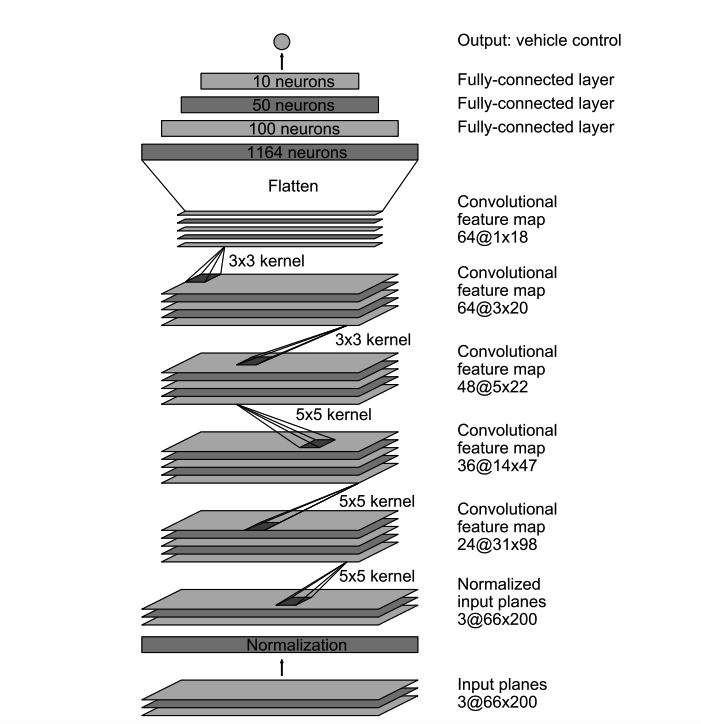
\includegraphics[width=\textwidth]{./imgs/NetworkOriginal.png}
			{\footnotesize Original architecture of the \textit{NVIDIA} paper \cite{NVIDIA2016}}
		\end{column}
	\end{columns}
\end{frame}

\begin{frame}{Our approaches to optimize the results}
	\begin{enumerate}
		\item \textbf{Change components of the initial architecture}
		\begin{itemize}
			\item Adding different pooling layers
			\item Use other activation functions
		\end{itemize}
		\item \textbf{Change the architecture}
		\begin{itemize}
			\item Expand structure to Siamese network
			\item Use different setups
		\end{itemize}
		\item \textbf{Change the input data}
		\begin{itemize}
			\item Acquire more data
			\item Use brightness augmentation
		\end{itemize}
	\end{enumerate}
\end{frame}